\documentclass[10pt,twoside]{article}
\usepackage{amsmath,amsthm,amsfonts,amssymb,bm,stmaryrd,pifont,mathtools,leftidx}
\usepackage{tikz}
\usetikzlibrary{arrows,backgrounds,shadows,decorations.markings,matrix}

\newcommand{\p}{\partial}
\newcommand{\df}{\mathsf{d}}

\begin{document}

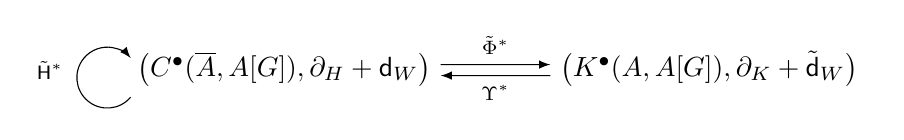
\begin{tikzpicture}
% Define the main matrix of complexes
\matrix (a) [matrix of math nodes, row sep=3.5em, column sep=4em, text height=2ex, text depth=0.9ex]
{\big(C^{\bullet}(\overline{A},A[G]),\p_H+\df_W\big) & \big(K^{\bullet}(A,A[G]),\p_K + \tilde{\df}_W\big)\\};

% Draw the self-loop on the left complex (homotopy operator)
\draw[-latex] (a-1-1.-170) arc (-40:-320:11pt);
\node[left, outer sep=20pt, font=\scriptsize] at (a-1-1.-180) {$\tilde{\mathsf{H}}^*$};

% Draw the forward quasi-isomorphism arrow
\path[-latex] (a-1-1.2) edge node[above, font=\scriptsize] {$\tilde{\Phi}^*$} (a-1-2.178.5);

% Draw the backward chain map arrow
\path[latex-] (a-1-1.-2) edge node[below, font=\scriptsize] {${\Upsilon}^*$} (a-1-2.-178.5);
\end{tikzpicture}

\end{document}